\section{Introduction}

In today's interconnected world, the abundance of information presents a significant challenge in measuring its transmission capacity. Enter Claude Elwood Shannon, a mathematician whose groundbreaking article revolutionized the field of communication and information. Shannon's Mathematical Theory of Communication introduced a systematic framework for quantifying the flow of information through a given system. In this article, we try to apply Shannon's theory to two different fields information compression and cryptography to see whether the outcomes align with our expectations.

\begin{figure}[!h]
\centering
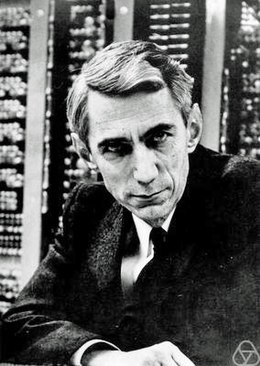
\includegraphics[scale=0.7]{images/shanon.jpg}
\caption{Claude Shannon around 1963 \cite{wiki_sha}}
\label{shannon}
\end{figure}

\newpage